In the section the approach followed to build the CCN will be described.
\subsection{Overall setup}
A deep CNN will be trained to give a probability distribution over the phonemes labels given the acoustic input. These probabilities will then be used to compute the emission probabilities of the HMM states in an CNN-HMM speech recognition system.
\subsection{Network Architecture}
As suggested in \cite{sainath2013deep}, a CNN network with both convolutional layers and fully connected layers cwill be used. The convolutional layers will be used at the lower layers of the network, while the fully. connected layers will be used at the top layers of the network. The convolutional layers will be followed with pooling layer. Having the convolutional layers at the bottom of the network helps with the spectral variation, and the fully connected layer are used to discriminate between the different phonemes using the convoluted-pooled input from the convolution and pooling layers.
\subsection{Feature representation}
As in \cite{graves2014towards} we have choosen to use the spectrograms as inputs to the CCN. The frames of the sound data of the  TIMIT corpus has been split into smaller chunks corresponding to the respective phonemes. The frames of each phoneme are then converted into a spectrogram and saved as an image. Figure \ref{fig:spect} shows an example spectrogram for a phoneme.
\begin{figure}[H]
\centering
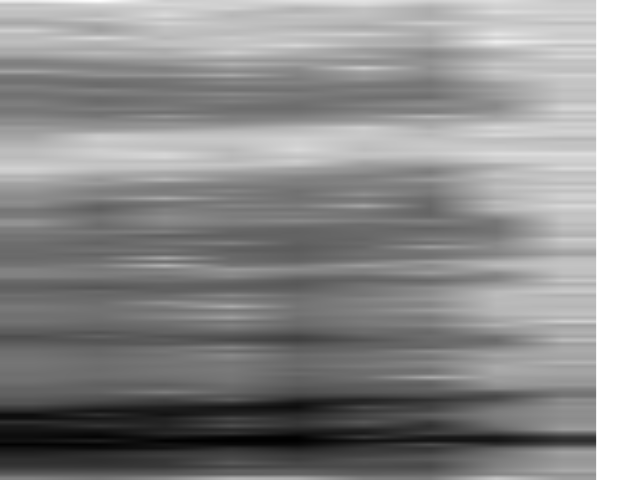
\includegraphics[width=1\linewidth]{figs/ah.png}
\caption{Spectrogram of phoneme \textbf{ah}}
\label{fig:spect}
\end{figure}
\subsection{Evaluation}
A number of CNN with different number of layers will be trained. The performance of these networks will be compared using the classification error rate. Due to the limitation of the computing resources, a relatively small networks will be trained, also the network will be trained to classify over a subset of the phonemes.